\chapter{Modello concettuale}\label{chp:modello-concettuale}
\begin{figure}[ht]
\centering
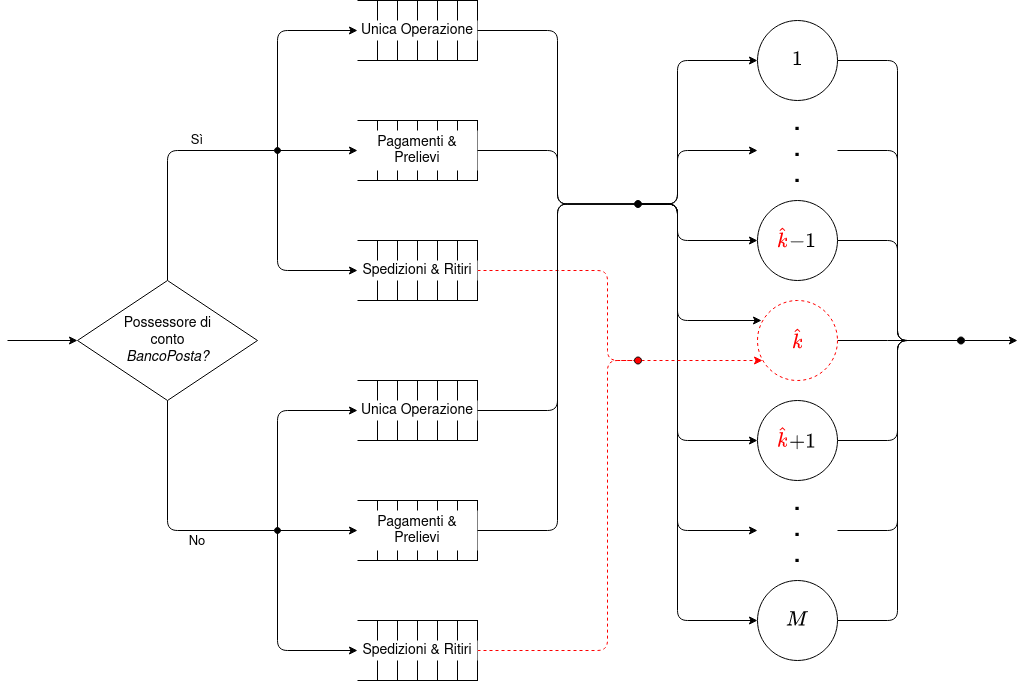
\includegraphics[width=\linewidth]{modello-concettuale-1}
\caption{Diagramma del sistema \textbf{Poste Italiane}}
\label{fig:modello-concettuale-1}
\end{figure}

Il funzionamento del sistema è illustrato dal diagramma in figura \ref{fig:modello-concettuale-1}. Di seguito è riportata una descrizione degli elementi in esso utilizzati:
\begin{itemize}
\item Il rombo rappresenta un meccanismo di ripartizione del flusso in ingresso nelle opportune code, a seconda della titolarità o meno di un conto \textsl{BancoPosta} da parte dei clienti.
\item Ciascuna coda modella una fila di clienti possessori dello stesso tipo di ticket.
\item Ciascun servente rappresenta uno sportello dell'ufficio postale
\begin{itemize}
\item Il $\ded$-esimo servente (evidenziato in {\color{red} rosso}) rappresenta lo sportello dedicato per la gestione dei ticket di tipo \sr{}, il cui comportamento è stato già illustrato nel flow chart in figura \ref{fig:presentazione-1}.
\end{itemize}
\end{itemize}

Ad ogni istante di tempo, lo stato del sistema è univocamente determinato dai valori assunti dalle seguenti $M + 12$ variabili di stato:
\begin{itemize}
\item Per ciascuno degli $M$ sportelli si ha:
\begin{equation}
Server_r \in
\left\lbrace \mathtt{IDLE},\ \mathtt{BUSY} \right\rbrace
\end{equation}
con $r \in \lbrace 1, 2, \dots, M \rbrace$.
\item Per ciascuna delle 6 classi di utenza:
\begin{itemize}
\item Il numero totale di clienti della $c-$esima è modellato dalla variabile $Customers_{c}$
\item Il numero di clienti in servizio della $c-$esima è modellato dalla variabile $InService_{c}$
\end{itemize}
con $c$ appartenente a:
\begin{multicols}{2}
\begin{itemize}
\item \uo{} \textsl{BancoPosta}
\item \pp{} \textsl{BancoPosta}
\item \sr{} \textsl{BancoPosta}
\item \uo{} \textsl{Standard}
\item \pp{} \textsl{Standard}
\item \sr{} \textsl{Standard}
\end{itemize}
\end{multicols}
\end{itemize}

Infine, si assume che:
\begin{itemize}
\item I clienti abbiano un comportamento di tipo \textsl{one-step}\footnote{Avere un comportamento di tipo \textsl{one-step} significa che vi può essere, ad ogni istante di tempo, lo spostamento di un solo cliente alla volta.}.
\item Non è possibile avere uno sportello libero se in coda è presente almeno un cliente con ticket processabile da tale sportello (sistema \textsl{work conserving}\footnote{La proprietà di \textsl{work conserving} è valida entro i vincoli imposti dal caso di studio.}).
\item All'inizio ed alla fine del periodo d'osservazione lo stato del sistema è il seguente:
\begin{equation}
\begin{cases}
Server_r =\mathtt{IDLE} & \forall\ r \\[1em]
Customers_{c} = \mathtt{NONE} & \forall\ c \\[1em]
InService_{c} = \mathtt{NONE} & \forall\ c
\end{cases}
\end{equation}
\end{itemize}